% Use only LaTeX2e, calling the article.cls class and 12-point type.

\documentclass[12pt]{article}

\usepackage{times}

% Packages I manually added
\usepackage{graphicx}
\usepackage{placeins}
\usepackage{float}
\usepackage{amsmath}
\usepackage{hyperref}

\topmargin 0.0cm
\oddsidemargin 0.2cm
\textwidth 16cm
\textheight 21cm
\footskip 1.0cm


% The preamble here sets up a lot of new/revised commands and
% environments.  It's annoying, but please do *not* try to strip these
% out into a separate .sty file (which could lead to the loss of some
% information when we convert the file to other formats).  Instead, keep
% them in the preamble of your main LaTeX source file.


% The following parameters seem to provide a reasonable page setup.

% Include your paper's title here

\title{Supplementary Materials for: ``Environmental Market Design for Large-Scale Marine Conservation''}


% Place the author information here.  Please hand-code the contact
% information and notecalls; do *not* use \footnote commands.  Let the
% author contact information appear immediately below the author names
% as shown.  We would also prefer that you don't change the type-size
% settings shown here.

\author{Juan Carlos Villase\~{n}or-Derbez,$^{1\ast}$ John Lynham,$^{2}$ Christopher Costello$^{1}$\\
\\
\normalsize{$^{1}$Bren School of Environmental Science \& Management,}\\
\normalsize{University of California at Santa Barbara, Santa Barbara, CA}\\
\normalsize{$^{2}$Department of Economics, University of Hawaii at Manoa, Honolulu, HI}\\
\\
\normalsize{$^\ast$To whom correspondence should be addressed; E-mail: juancarlos@ucsb.edu.}
}

% Include the date command, but leave its argument blank.

\date{}



%%%%%%%%%%%%%%%%% END OF PREAMBLE %%%%%%%%%%%%%%%%

\begin{document}

% Double-space the manuscript.

\baselineskip24pt

% Make the title.

\maketitle

\newcommand{\beginsupplement}{\setcounter{table}{0}  \renewcommand{\thetable}{S\arabic{table}} \setcounter{figure}{0} \renewcommand{\thefigure}{S\arabic{figure}}}

\setcounter{table}{0}  \renewcommand{\thetable}{S\arabic{table}} \setcounter{figure}{0} \renewcommand{\thefigure}{S\arabic{figure}}

\section{Model parameterization}

We calibrate our model to loosely match the fishery dynamics observed for the VDS operated by the PNA. The table below contains the values used to parameterize the model.

\begin{table}[H]
	
	\caption{\label{tab:param_table}Model parameters.}
\centering
\resizebox{\linewidth}{!}{
\begin{tabular}{l|r|l}
\hline
Parameter & Value & Source\\
\hline
MSY & 1.875600e+06 & 50th percentile from MSY in Table 8 of WCPFC Stock Assessment\\
\hline
$B_{msy}$ & 1.628000e+06 & 50th percentile from MSY in Table 8 of WCPFC Stock Assessment\\
\hline
K & 6.876526e+06 & 50th percentile from MSY in Table 8 of WCPFC Stock Assessment\\
\hline
$B_c/B_{msy}$ & 0.51 & 50th percentile from MSY in Table 8 of WCPFC Stock Assessment\\
\hline
$C_{now}$ & 1.679444e+06 & Catches from WCPFC Stock Assessment\\
\hline
$B_{now}$ & 3.507028e+06 & Current Biomass (2012 - 2015 average)\\
\hline
$r$ & 0.57 & From FishBase: Prior r = 0.57, 95 CL = 0.41 - 0.78\\
\hline
$\beta$ & 1.3 & Standard \cite{costello_2016}\\
\hline
p & 1100 & Mean between Thailand and Japan values (Value of WCPFC-CA Tuna Fisheries 2017 Report)\\
\hline
q & 3.420000e-05 & Estimated so that efforts match catches given biomass and vessel-day prices\\
\hline
c & 1800 & Estimated to match cost and revenue structures\\
\hline
f & 0.1 & Biomass is equally distributed between countries\\
\hline
\end{tabular}}
\end{table}


\section{Balance on observables}

We observe six characteristics for every vessel: flag, crew size, engine power, vessel length, tonnage capacity, and fishing hours within PNA waters in 2014. Figure \ref{fig:balance_density_plot} shows the distribution of the numeric variables for each group of vessels. Table \ref{tab:balance_table} presents the mean and standard deviation of each observable, and table \ref{tab:balance_table_flags} shows the composition of each group by flag. On average, displaced vessels have smaller crew sizes, more engine power, are larger than non-displaced vessels, and fished more in PNA waters during 2014. The largest relative difference is in terms of gross tonnage. 

%% TABLE FOR NUMERIC VARIALBES
\begin{table}[H]
\caption{\label{tab:balance_table}Mean values on observable characteristics by vessel for displaced (n = 64), and non-displaced vessels (n = 254). Numbers in parentheses indicate standard deviation. The last column contains the difference in means (t-scores), with asterisks indicating significant differences as indicated by a two-tailed t-test (* p $<$ 0.1; ** p $<$ 0.05; *** p $<$ 0.01).}
\centering
\begin{tabular}{l|l|l|l}
\hline
Characteristic & Displaced & Non-displaced & Difference\\
\hline
Crew size (n) & 26.38 (3.94) & 30.46 (6.25) & 4.08 (6.49) ***\\
\hline
Engine Power (KW) & 2983.6 (558.76) & 2559.89 (588.28) & -423.71 (-5.36) ***\\
\hline
Length (m) & 74.23 (9.71) & 68.97 (8.42) & -5.25 (-3.97) ***\\
\hline
PNA fishing in 2014 (hours) & 667.57 (489.24) & 529.33 (380.11) & -138.24 (-1.89) *\\
\hline
Tonnage (GT) & 1718.14 (653.38) & 1383.41 (533.56) & -334.73 (-3.79) ***\\
\hline
\end{tabular}
\end{table}

%% BALANCE TABLE FOR FLAGS
\begin{table}[t]
\caption{\label{tab:balance_table_flags}Proportion of vessel flags by group. Note that we do not observe the flag for two vessels (0.78\%) in the non-displaced group.}
\centering
\begin{tabular}{l|r|r}
\hline
Flag & Non-displaced & Displaced\\
\hline
CHN & 10.24 & 0.00\\
\hline
ECU & 1.57 & 4.69\\
\hline
ESP & 0.39 & 4.69\\
\hline
FSM & 8.27 & 3.12\\
\hline
GTM & 0.39 & 1.56\\
\hline
JPN & 16.93 & 0.00\\
\hline
KIR & 2.76 & 12.50\\
\hline
KOR & 3.54 & 45.31\\
\hline
MEX & 1.18 & 0.00\\
\hline
MHL & 3.54 & 1.56\\
\hline
NIC & 0.39 & 0.00\\
\hline
NRU & 0.39 & 0.00\\
\hline
NZL & 1.18 & 3.12\\
\hline
PAN & 0.79 & 0.00\\
\hline
PHL & 7.87 & 1.56\\
\hline
PNG & 11.42 & 1.56\\
\hline
SLB & 1.57 & 0.00\\
\hline
SLV & 0.79 & 0.00\\
\hline
TWN & 11.81 & 3.12\\
\hline
USA & 12.20 & 17.19\\
\hline
VUT & 1.97 & 0.00\\
\hline
Not reported & 0.79 & 0.00\\
\hline
Total & 100.00 & 100.00\\
\hline
\end{tabular}
\end{table}

\clearpage

\FloatBarrier

\section{Supplementary figures}

\begin{figure}[htbp]
\centering
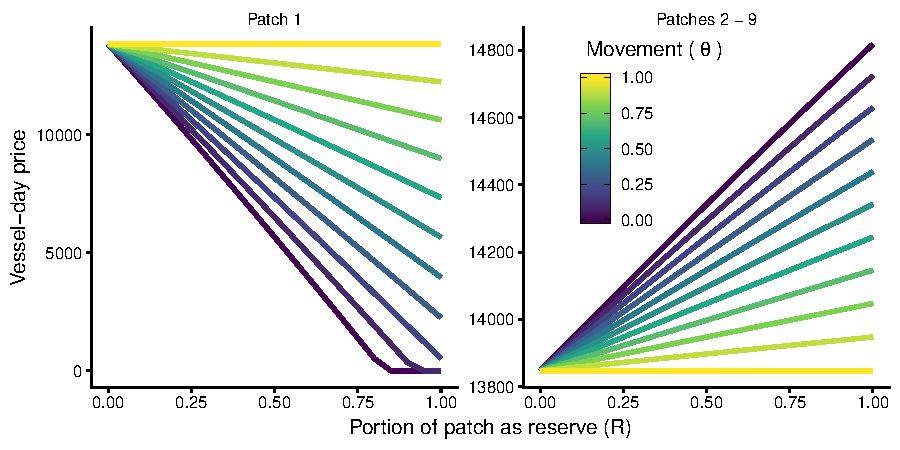
\includegraphics{img/vessel_day_price_no_trading_plot.pdf}
\caption{\label{fig:vessel_day_price_no_trading_plot}Vessel-day prices (vertical axis) for a combination of reserve sizes ($R$ in the horizontal-axis) and different within-country movement ($\theta$) for the country with spatial closure and other countries (left - right, respectively) when there is no trading.}
\end{figure}

\begin{figure}[htbp]
\centering
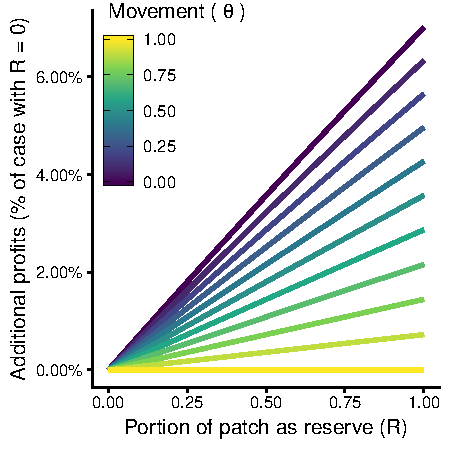
\includegraphics{img/profits_PNA_notKIR_no_trading_plot.pdf}
\caption{\label{fig:profits_PNA_notKIR_no_trading_plot}Relative change in revenue for countries 2 - 9 (vertical axis) for a combination of reserve sizes ($R$ in the horizontal-axis) and different within-country movement ($\theta$) when there is no trading.}
\end{figure}

\begin{figure}
\centering
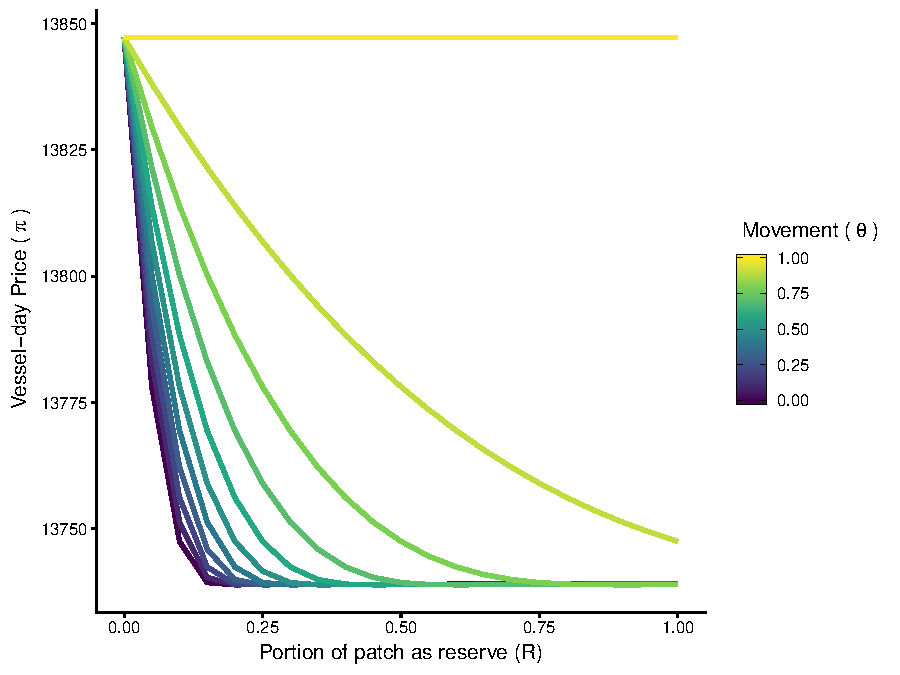
\includegraphics{img/vessel_day_price_with_trading_plot.pdf}
\caption{\label{fig:vessel_day_price_with_trading_plot}PNA-wide vessel-day prices (vertical axis) with trading, for a combination of reserve sizes ($R$ in the horizontal-axis) and different within-country movement ($\theta$).}
\end{figure}

\begin{figure}
	\centering
	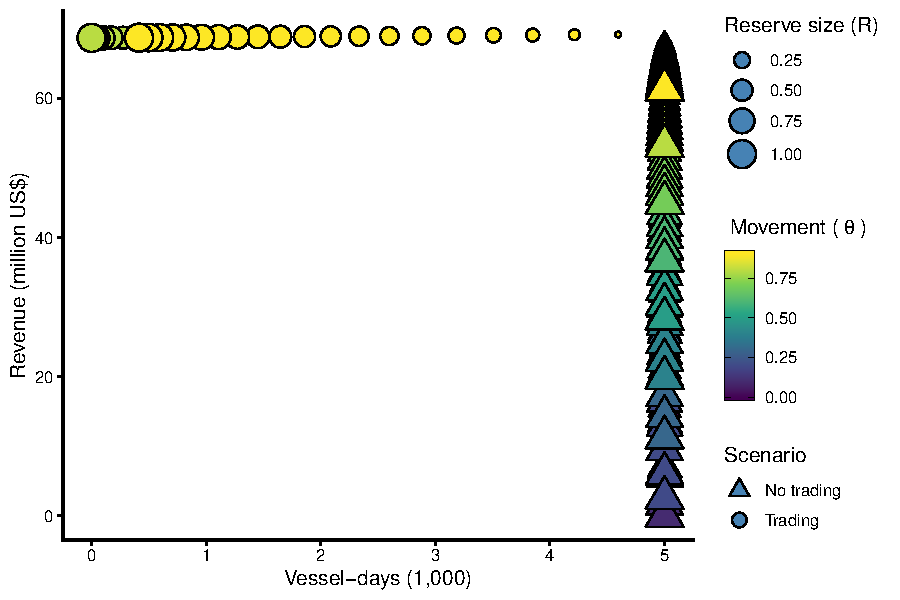
\includegraphics{img/effort_and_revenues.pdf}
	\caption{\label{fig:effort_and_revenues}Effort and revenue in Country 1 for a combination of reserve sizes ($R$), different within-country movement ($\theta$), and with and without trading. With trading, the relative drop in effort is always larger than the relative drop in revenue as $R$ increases. The exact opposite relationship holds without trading: effort remains fixed as revenue declines with increasing $R$.}
\end{figure}

\begin{figure}
\centering
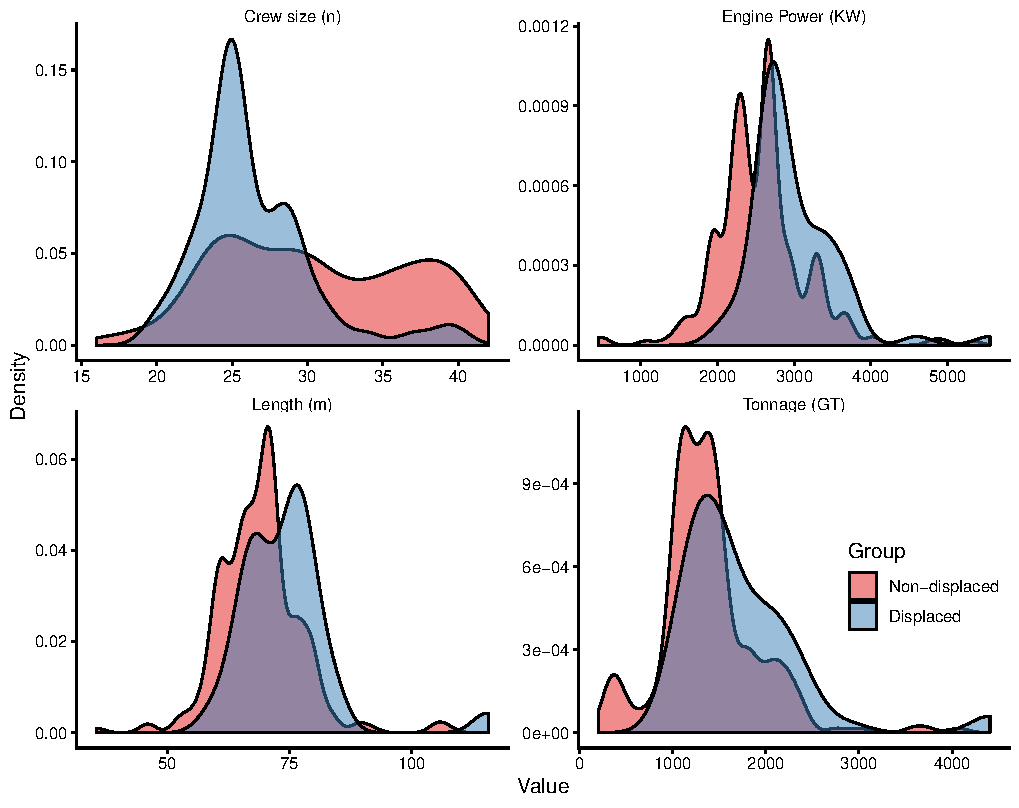
\includegraphics{img/balance_density_plot.pdf}
\caption{\label{fig:balance_density_plot}Distribution of observable characteristics by vessel for displaced (n = 64), non-displaced vessels (n = 254).}
\end{figure}

\begin{figure}
\centering
	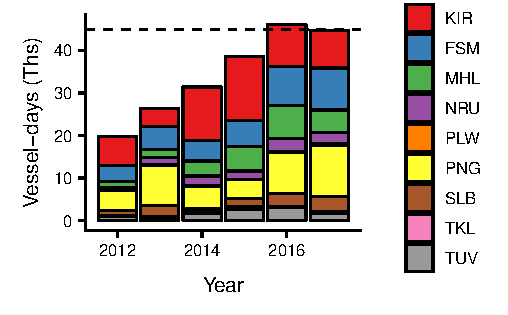
\includegraphics{img/all_PS_VDS_cty_year.pdf}
	\caption{\label{fig:all_PS_VDS_cty_year}Annual country-level vessel-days for all PNA countries by 318 tuna purse seiners.}
\end{figure}

\begin{figure}
\centering
	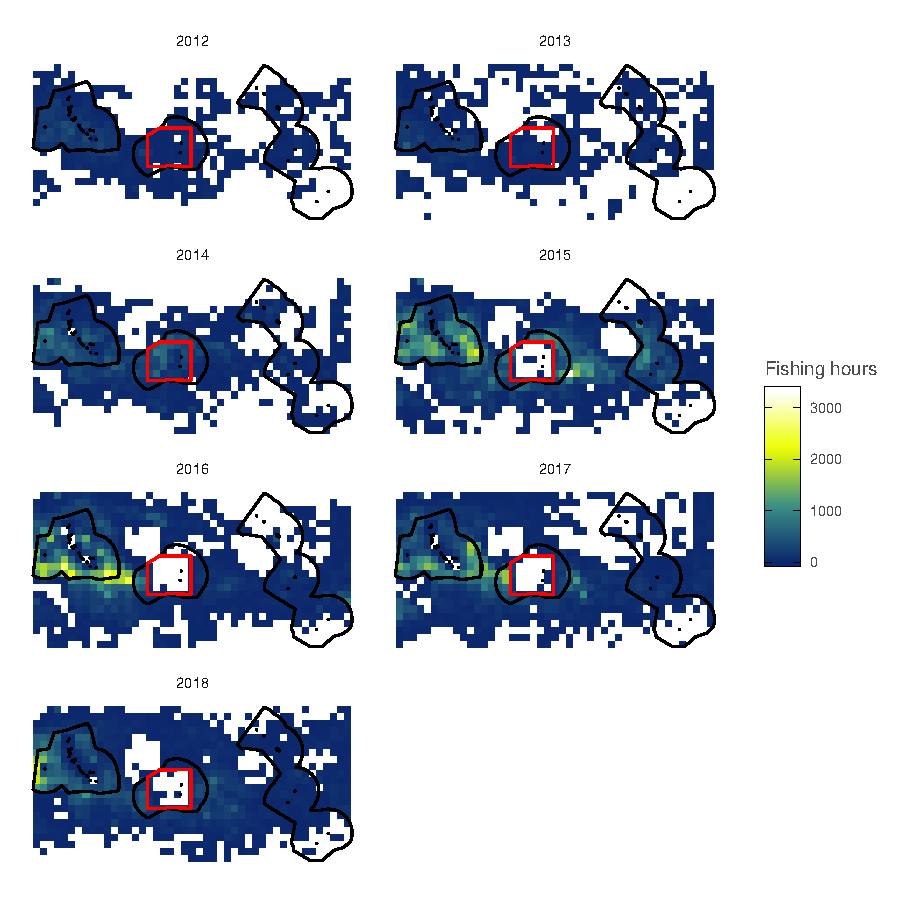
\includegraphics{img/fishing_the_line_by_year.pdf}
	\caption{\label{fig:fishing_the_line_by_year}Annual fishing effort (hours) on a 1-degree grid around PIPA (red polygon) and Kiribati (black polygons). There is no clear evidence of a ``fishing the line'' effect, with the greatest effort applied on the Gilbert islands (Kiribati) after 2015.}	
\end{figure}

\begin{figure}
\centering
	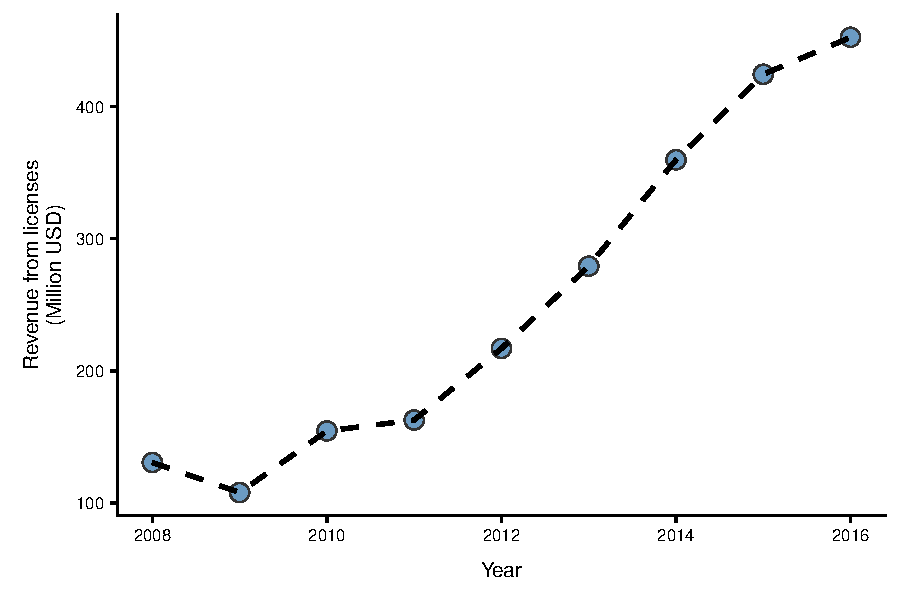
\includegraphics{img/total_PNA_revenues.pdf}
	\caption{\label{fig:total_PNA_revenues}Total revenues for all PNA countries combined.}
\end{figure}

\begin{figure}
\centering
	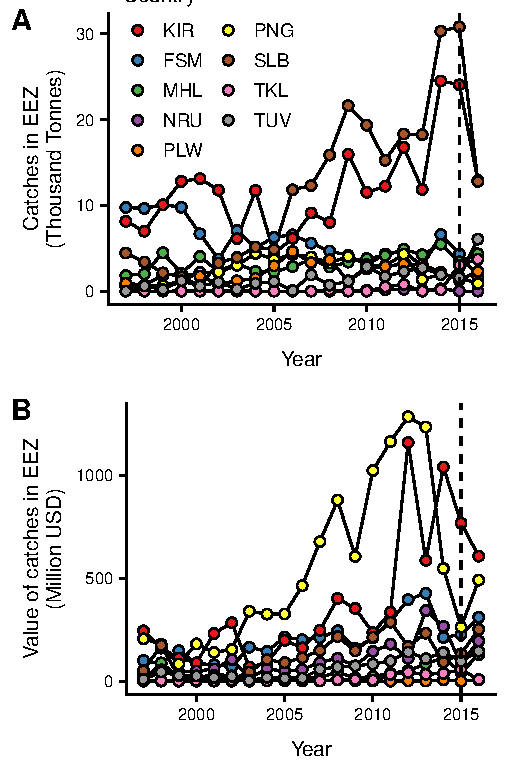
\includegraphics{img/catches.pdf}
	\caption{\label{fig:catches}Financial indicators for PNA countries. A) Total annual purse seine catch by EEZ and, B) Total annual value of purse seine catch by EEZ. Vertical dashed line in both plots denotes implementation of PIPA.}
\end{figure}

\begin{figure}
\centering
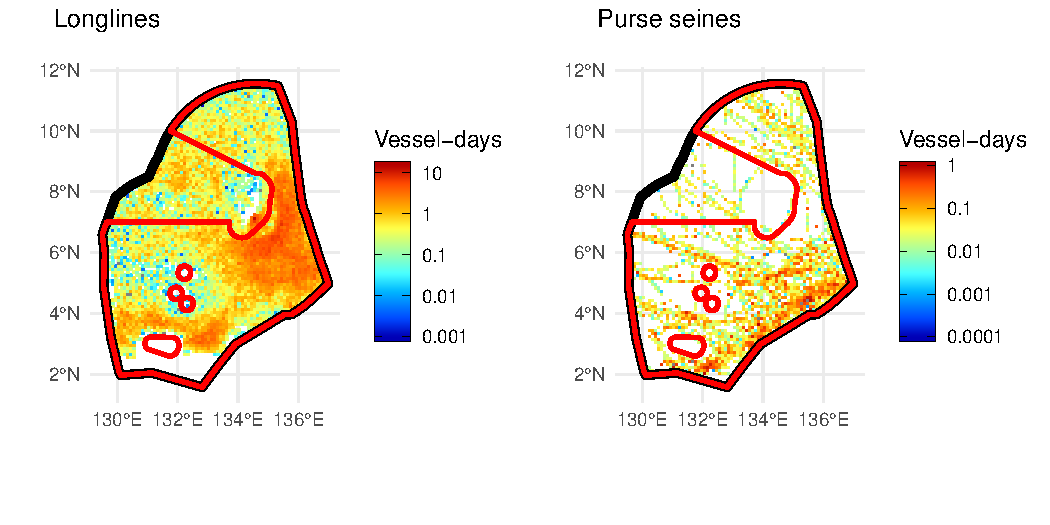
\includegraphics{img/plw_2018.pdf}
\caption{\label{fig:plw_2018}Longline and purse seine fishing effort in Palau during 2018 at a 0.5 degree resolution. The red polygon shows the proposed Palau National Marine Sanctuary, containing 56\% and 91\% of longline and purse seine fishing effort, respectively. Note that the colorbars are presented in $log_{10}$ transformed scale for better visualization.}
\end{figure}

\begin{figure}
\centering
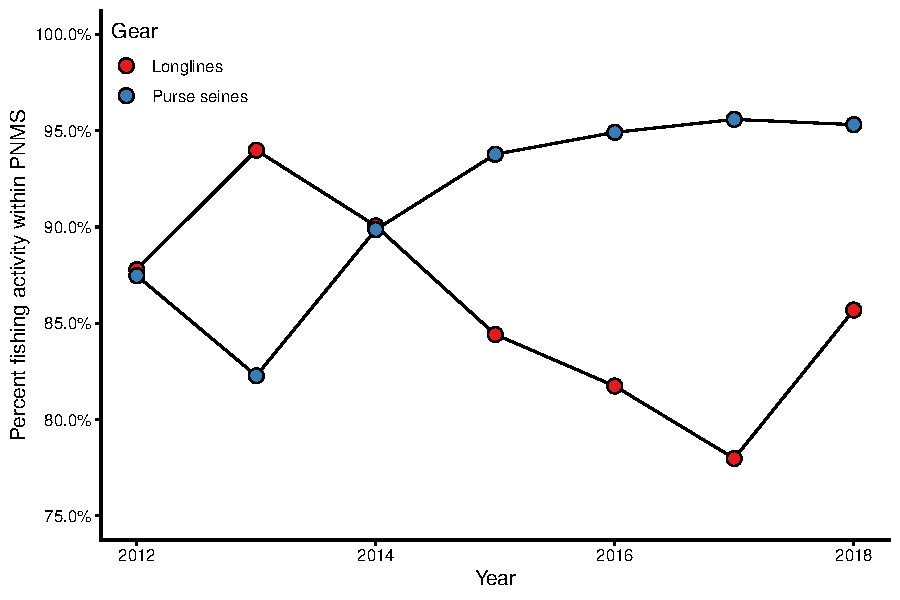
\includegraphics{img/plw_ts_plot.pdf}
\caption{\label{fig:plw_ts_plot}Time series of the annual proportion of longline and purse seine effort within the proposed PNMS boundaries.}
\end{figure}

\clearpage

\bibliography{references}
\bibliographystyle{nature}

\end{document}
